%\documentclass[11pt]{article}
%\usepackage{sw20jart}
%\input{tcilatex}


\documentclass[11pt]{article}
%%%%%%%%%%%%%%%%%%%%%%%%%%%%%%%%%%%%%%%%%%%%%%%%%%%%%%%%%%%%%%%%%%%%%%%%%%%%%%%%%%%%%%%%%%%%%%%%%%%%%%%%%%%%%%%%%%%%%%%%%%%%%%%%%%%%%%%%%%%%%%%%%%%%%%%%%%%%%%%%%%%%%%%%%%%%%%%%%%%%%%%%%%%%%%%%%%%%%%%%%%%%%%%%%%%%%%%%%%%%%%%%%%%%%%%%%%%%%%%%%%%%%%%%%%%%
\usepackage{natbib}
\usepackage{setspace}
\usepackage[left=2.5cm,top=2.8cm,right=2.5cm,bottom=2.8cm]{geometry}
\usepackage{graphicx}
\usepackage{amsmath}
\usepackage{theorem}
\usepackage{version}
\usepackage{multirow}
\usepackage{amssymb}
\usepackage{tikz}
\usetikzlibrary{arrows,arrows.meta,decorations,decorations.pathreplacing,calc,matrix}

\definecolor{Red}{rgb}{1,0,0}
\definecolor{Blue}{rgb}{0,0,1}
\definecolor{Green}{rgb}{0,1,0}
\definecolor{magenta}{rgb}{1,0,.6}
\definecolor{lightblue}{rgb}{0,.5,1}
\definecolor{lightpurple}{rgb}{.6,.4,1}
\definecolor{gold}{rgb}{.6,.5,0}
\definecolor{orange}{rgb}{1,0.4,0}
\definecolor{hotpink}{rgb}{1,0,0.5}
\definecolor{newcolor2}{rgb}{.5,.3,.5}
\definecolor{newcolor}{rgb}{0,.3,1}
\definecolor{newcolor3}{rgb}{1,0,.35}
\definecolor{darkgreen1}{rgb}{0, .35, 0}
\definecolor{darkgreen}{rgb}{0, .6, 0}
\definecolor{darkred}{rgb}{.75,0,0}
\definecolor{lightgrey}{rgb}{.7,.7,.7}

\definecolor{clemson-orange}{RGB}{234,106,32}
\definecolor{chicago-maroon}{RGB}{128,0,0}
\definecolor{northwestern-purple}{RGB}{82,0,99}
\definecolor{cornell-red}{RGB}{179,27,27}
\definecolor{sauder-green}{RGB}{171,180,0}
%\definecolor{gray}{RGB}{192,192,192}
\definecolor{lawngreen}{RGB}{0,250,154}

\setcounter{MaxMatrixCols}{10}

\onehalfspacing
\newtheorem{theorem}{Theorem}
\newtheorem{acknowledgement}{Acknowledgement}
\newtheorem{algorithm}{Algorithm}
\newtheorem{assumption}{Assumption}
\newtheorem{axiom}{Axiom}
\newtheorem{case}{Case}
\newtheorem{claim}{Claim}
\newtheorem{conclusion}{Conclusion}
\newtheorem{condition}{Condition}
\newtheorem{conjecture}{Conjecture}
\newtheorem{corollary}{Corollary}
\newtheorem{criterion}{Criterion}
\newtheorem{definition}{Definition}
\newtheorem{example}{Example}
\newtheorem{exercise}{Exercise}
\newtheorem{lemma}{Lemma}
\newtheorem{notation}{Notation}
\newtheorem{problem}{Problem}
\newtheorem{proposition}{Proposition}
{\theorembodyfont{\normalfont}
\newtheorem{remark}{Remark}
}
\newtheorem{summary}{Summary}
\newenvironment{proof}[1][Proof]{\textbf{#1.} }{\hfill \rule{0.5em}{0.5em} \bigskip}
\newenvironment{soln}[1][Soln]{\textbf{#1:} }{\hfill \rule{0.5em}{0.5em}}
\renewcommand{\cite}{\citeasnoun}
\renewcommand{\theenumii}{(\alph{enumii})}
\renewcommand{\labelenumii}{\theenumii}
\renewcommand{\theenumiii}{\roman{enumiii}}
\renewcommand{\labelenumiii}{\theenumiii.}

\usepackage[nameinlink]{cleveref}
\crefname{assumption}{Assumption}{Assumptions}
\crefname{lemma}{Lemma}{Lemmas}
\crefname{theorem}{Theorem}{Theorems}
\crefname{corollary}{Corollary}{Corollaries}
\crefname{proposition}{Proposition}{Propositions}
\crefname{claim}{Claim}{Claims}
\crefname{procedure}{Procedure}{Procedures}
\crefname{algorithm}{Algorithm}{Algorithms}
\crefname{figure}{Figure}{Figures}
\crefname{remark}{Remark}{Remarks}
\crefname{section}{Section}{Sections}
\crefname{procedure}{Procedure}{Procedures}
\crefname{example}{Example}{Examples}
\crefname{definition}{Definition}{Definitions}
\crefname{table}{Table}{Tables}
\crefname{align}{}{}
\crefname{enumi}{}{}
\crefname{conjecture}{Conjecture}{Conjectures}
\crefname{step}{Step}{Steps}
\crefname{appendix}{Appendix}{Appendices}
\crefname{footnote}{Footnote}{Footnotes}

\begin{document}


\begin{center}
\textbf{ECON 201 Week 14 Problem Set}\\
\textit {Professor: Teddy kim};  
Sunday, December 2nd.
\\Student name: Hridansh Saraogi
\end{center}

\begin{enumerate}
\item For each of the following statements, determine whether
the statement is \emph{true} or \emph{false} (the latter including ``not necessarily true''), and provide a brief explanation.
    \begin{enumerate}
    \item A situation where everyone is playing a dominant strategy must be a Nash equilibrium.
    \begin{enumerate}
        \item T
        \item Dominant Strategy: all of your best responses agree
    \end{enumerate}

    \item In a Nash equilibrium, everyone must be playing a dominant strategy.
    \begin{enumerate}
        \item 
    \end{enumerate}

    \item A two-person game in which each person has access to only two possible strategies will have at most one Nash equilibrium.
    \begin{enumerate}
        \item 
    \end{enumerate}

    \item In the following game, there exists only one pure-strategy equilibrium.
        \begin{figure}[h!]
    \begin{center}
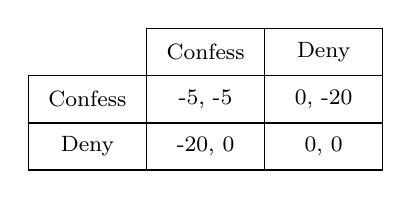
\begin{tikzpicture}[scale=0.6]
	
	\draw[line width=0.5pt] (2.5,2) rectangle node{\footnotesize{Confess}} (5,1);
	\draw[line width=0.5pt] (2.5,1) rectangle node{\footnotesize{Deny}} (5,0);

    \draw[line width=0.5pt] (5,3) rectangle node{\footnotesize{Confess}} (7.5,2);
    \draw[line width=0.5pt] (7.5,3) rectangle node{\footnotesize{Deny}} (10,2);

    \draw[line width=0.5pt] (5,2) rectangle node{\footnotesize{-5,~-5}} (7.5,1);
    \draw[line width=0.5pt] (5,1) rectangle node{\footnotesize{-20,~0}} (7.5,0);
    \draw[line width=0.5pt] (7.5,2) rectangle node{\footnotesize{0,~-20}} (10,1);
    \draw[line width=0.5pt] (7.5,1) rectangle node{\footnotesize{0,~0}} (10,0);
    	
	\end{tikzpicture}
\end{center}
    \end{figure}
    \begin{enumerate}
        \item 
    \end{enumerate}

    \item In the following game of matching pennies, if player 2 plays $(1/2\circ H,1/2\circ T)$ (i.e., plays both strategies with equal probability) then player 1 strictly prefers playing $(1/2\circ H,1/2\circ T)$ to playing either $H$ or $T$ with probability 1.

    \begin{center}
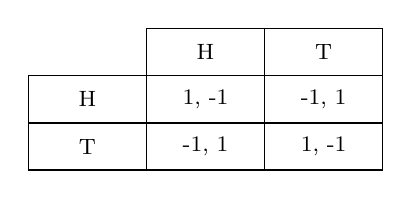
\begin{tikzpicture}[scale=0.6]
	
	\draw[line width=0.5pt] (2.5,2) rectangle node{\footnotesize{H}} (5,1);
	\draw[line width=0.5pt] (2.5,1) rectangle node{\footnotesize{T}} (5,0);

    \draw[line width=0.5pt] (5,3) rectangle node{\footnotesize{H}} (7.5,2);
    \draw[line width=0.5pt] (7.5,3) rectangle node{\footnotesize{T}} (10,2);

    \draw[line width=0.5pt] (5,2) rectangle node{\footnotesize{1,~-1}} (7.5,1);
    \draw[line width=0.5pt] (5,1) rectangle node{\footnotesize{-1,~1}} (7.5,0);
    \draw[line width=0.5pt] (7.5,2) rectangle node{\footnotesize{-1,~1}} (10,1);
    \draw[line width=0.5pt] (7.5,1) rectangle node{\footnotesize{1,~-1}} (10,0);

	\end{tikzpicture}
\end{center}
    \begin{enumerate}
        \item 
    \end{enumerate}
	\end{enumerate}

\item In each of the following games, find all pure-strategy and mixed-strategy Nash equilibria.
    \begin{enumerate}
    \item Battle of the sexes:
    \begin{figure}[h!]
    \begin{center}
    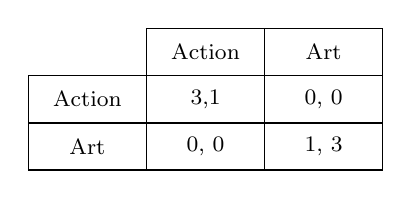
\begin{tikzpicture}[scale=0.6]
	
	\draw[line width=0.5pt] (2.5,2) rectangle node{\footnotesize{Action}} (5,1);
	\draw[line width=0.5pt] (2.5,1) rectangle node{\footnotesize{Art}} (5,0);

    \draw[line width=0.5pt] (5,3) rectangle node{\footnotesize{Action}} (7.5,2);
    \draw[line width=0.5pt] (7.5,3) rectangle node{\footnotesize{Art}} (10,2);

    \draw[line width=0.5pt] (5,2) rectangle node{\footnotesize{3,1}} (7.5,1);
    \draw[line width=0.5pt] (5,1) rectangle node{\footnotesize{0,~0}} (7.5,0);
    \draw[line width=0.5pt] (7.5,2) rectangle node{\footnotesize{0,~0}} (10,1);
    \draw[line width=0.5pt] (7.5,1) rectangle node{\footnotesize{1,~3}} (10,0);
    	
	\end{tikzpicture}
\end{center}
    \end{figure}

    \item Game of Chicken:
	\begin{figure}[h!]
    \begin{center}
    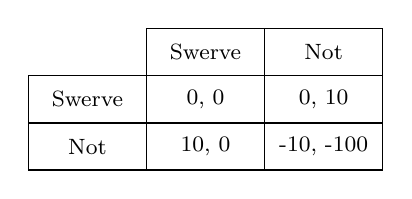
\begin{tikzpicture}[scale=0.6]
	
	\draw[line width=0.5pt] (2.5,2) rectangle node{\footnotesize{Swerve}} (5,1);
	\draw[line width=0.5pt] (2.5,1) rectangle node{\footnotesize{Not}} (5,0);

    \draw[line width=0.5pt] (5,3) rectangle node{\footnotesize{Swerve}} (7.5,2);
    \draw[line width=0.5pt] (7.5,3) rectangle node{\footnotesize{Not}} (10,2);

    \draw[line width=0.5pt] (5,2) rectangle node{\footnotesize{0,~0}} (7.5,1);
    \draw[line width=0.5pt] (5,1) rectangle node{\footnotesize{10,~0}} (7.5,0);
    \draw[line width=0.5pt] (7.5,2) rectangle node{\footnotesize{0,~10}} (10,1);
    \draw[line width=0.5pt] (7.5,1) rectangle node{\footnotesize{-10,~-100}} (10,0);
    	
	\end{tikzpicture}
\end{center}
    \end{figure}

	\end{enumerate}

\item Player 1 is a potential entrant into a market dominated by player 2 (incumbent). Initially, player 1 decides whether to go in or stay out. If player 1 stays out, then player 2 enjoys the highest payoff ($2$); player 1 obtains a modest payoff ($1$). If player 1 chooses to come in, then player 2 decides whether to fight or acquiesce. If player 2 acquiesces, then player 1 obtains the highest payoff ($2$), while player 2 receives a modest payoff ($1$). If player 2 fights, however, then both players suffer and receive the worst payoff ($0$).

\begin{center}
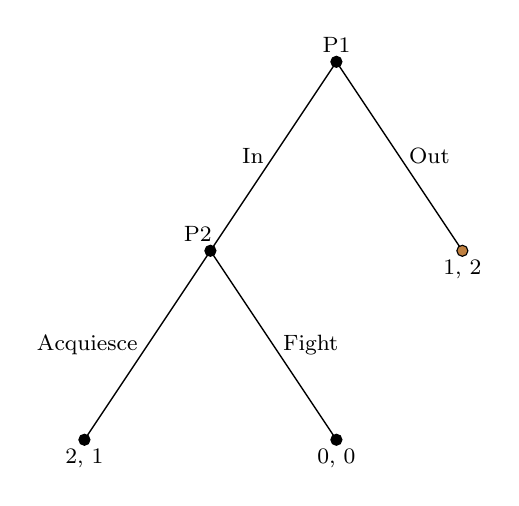
\begin{tikzpicture}[scale=0.8]
		
    \draw[fill=black] (3,6) circle (2.5pt);
	\fill (3,6) node[above] {\footnotesize{P1}};
	
	\draw[line width=0.5pt,black] (3,6)--(1,3);
	\fill (2,4.5) node[left] {\footnotesize{In}};
	
	\draw[line width=0.5pt,black] (3,6)--(5,3);
	\fill (4,4.5) node[right] {\footnotesize{Out}};
	
	\draw[fill=brown] (5,3) circle (2.5pt);
	\fill (5,3) node[below] {\footnotesize{1,~2}};
	
	\fill (0.8,3) node[above] {\footnotesize{P2}};
	\draw[fill=black] (1,3) circle (2.5pt);
	
	\draw[line width=0.5pt,black] (1,3)--(-1,0);
	\draw[line width=0.5pt,black] (1,3)--(3,0);
	
	\draw[fill=black] (-1,0) circle (2.5pt);
	\draw[fill=black] (3,0) circle (2.5pt);
	
	\fill (0,1.5) node[left] {\footnotesize{Acquiesce}};
	\fill (2,1.5) node[right] {\footnotesize{Fight}};
	
	\fill (-1,0) node[below] {\footnotesize{2,~1}};
	\fill (3,0) node[below] {\footnotesize{0,~0}};
		
\end{tikzpicture}
\end{center}

	\begin{enumerate}
	\item Show that (In, Acquiesce) is a Nash equilibrium of this game.
	
	\item Show that (Out, Fight) is also a Nash equilibrium of this game.
	

	\item Show that (Out, Fight) is not a subgame perfect Nash equilibrium.
	\end{enumerate}

\end{enumerate}

\end{document}


